\documentclass[a4paper,12pt]{report}

\usepackage{alltt, fancyvrb, url}
\usepackage{graphicx}
\usepackage[utf8]{inputenc}
\usepackage{float}
\usepackage{hyperref}

% Questo commentalo se vuoi scrivere in inglese.
\usepackage[italian]{babel}

\usepackage[italian]{cleveref}

\title{Report progetto\\``Puzzle Bobble''}

\author{Riccardo Pepe\\
		Beatrice Barba}
\date{\today}


\begin{document}

\maketitle

\tableofcontents

\chapter{Analisi}

\section{Requisiti}

Il software che si vuole realizzare mira alla costruzione di un gioco rompicapo su livelli ispirato al famoso ``Puzzle Bubble''. 
Il gioco consiste nel liberare, tramite un cannone al cui interno è posizionata una pallina dal colore casuale, un tabellone che presenta un pattern delle suddette sfere.  Per superare il livello bisognerà liberare quest'ultimo dalle palline colorate prima che le sfere superino un punto limite e quindi venga dichiarato il game over.


\subsubsection{Requisiti funzionali}
\begin{itemize}
	\item Quando si formano degli agglomerati di minimo 3 sfere dello stesso colore, queste esploderanno incrementando il punteggio, facendo cadere anche le altre sottostanti che si ancoravano ad esso.
	\item Per liberare il tabellone è necessario far esplodere tutte le palline presenti.
	\item Dopo un determinato numero di colpi la difficoltà del giocatore nel liberare l'intero tabellone verrà incrementata gradualmente.
	\item Al completamento di ogni livello il gioco si occuperà di salvare automaticamente lo stato del gioco
\end{itemize}

\subsubsection{Requisiti non funzionali}
\begin{itemize}
	\item Il gioco deve rimanere fluido in tutte le sue fasi
\end{itemize}

\section{Analisi e modello del dominio}

Il gioco si compone di un tabellone rettangolare dove, nella parte alta, vengono posizionate delle palline in base ad uno schema; queste, in base al loro colore, possiedono punteggi differenti che, una volta esplose, incrementeranno il punteggio del giocatore. Nella parte inferiore dell'area di gioco è situato al centro un cannone al cui interno è presente una sfera dal colore casuale. L'utente può modificare la direzione del cannone e decidere dove sparare la pallina, tenendo conto che essa può rimbalzare sulle pareti laterali del rettangolo. Durante la partita, dopo un determinato numero di colpi effettuati, dalla parte superiore del tabellone inizierà a scendere un muro che avvicinerà le palline al cannone, aumentando così la difficoltà del livello. Il game over avviene quando le sfere inesplose superano una determinata linea di demarcazione. 

\begin{figure}[H]
\centering{}
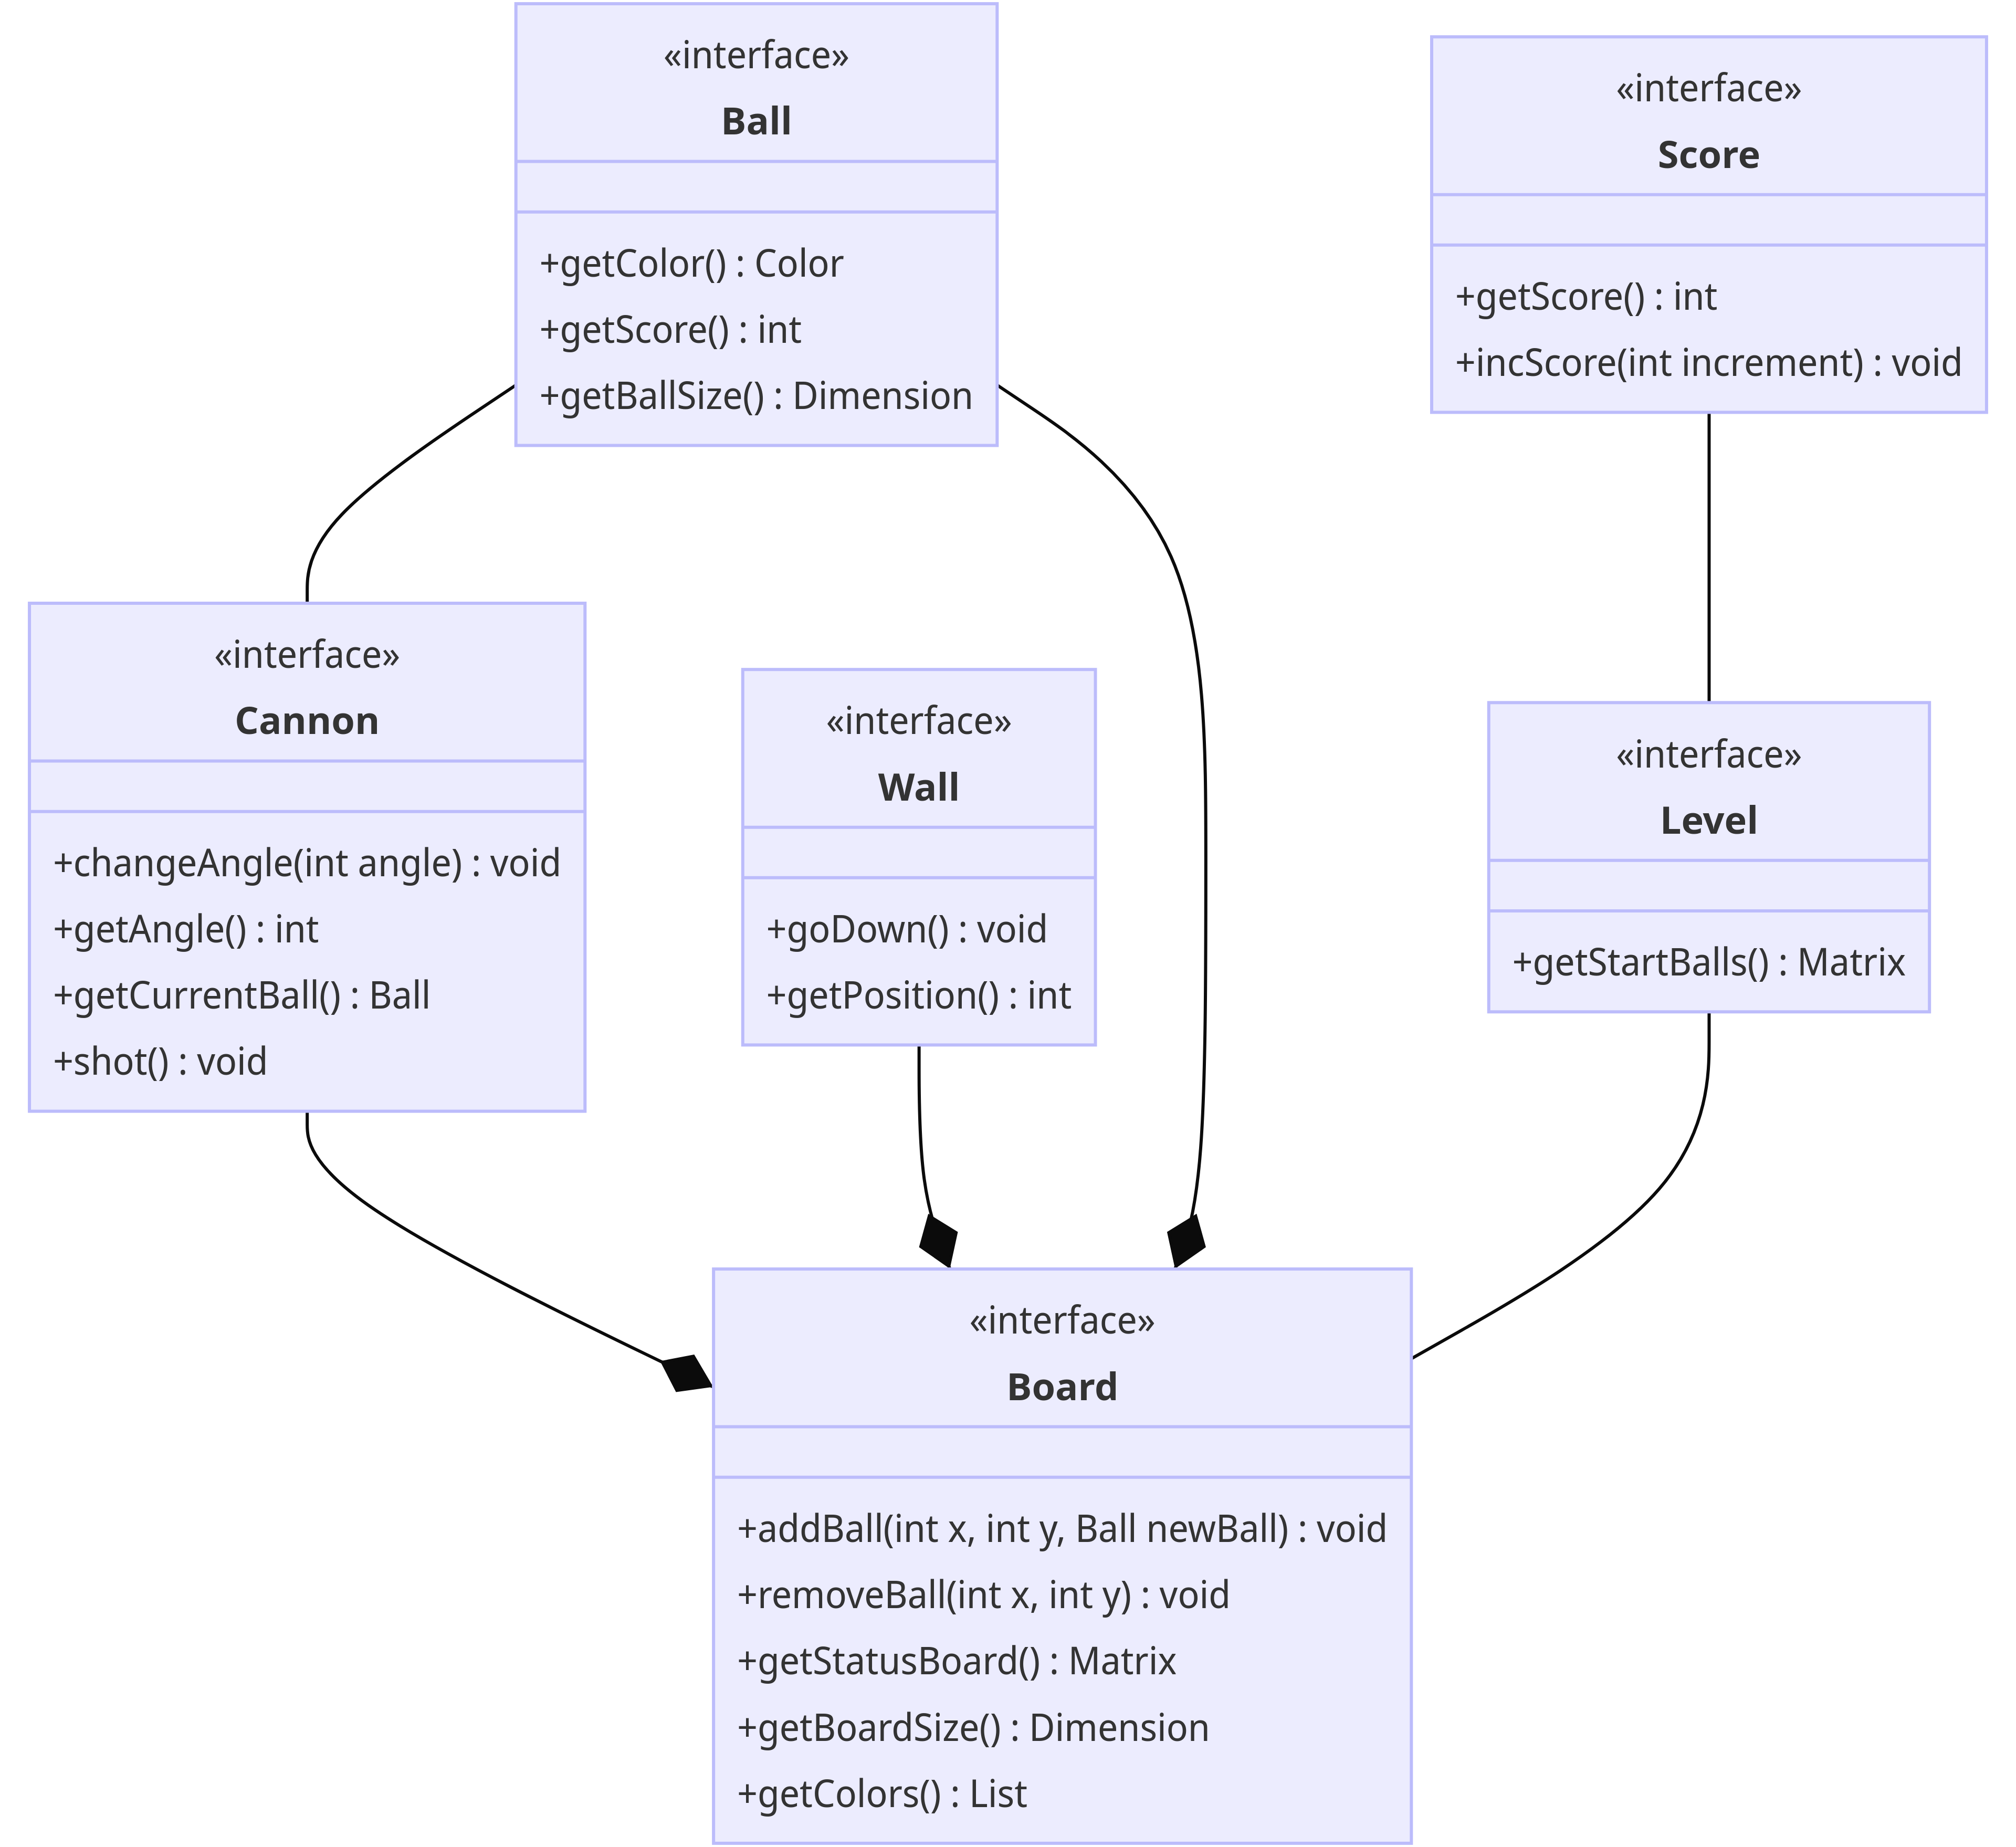
\includegraphics[width=\textwidth]{img/Diagramma_UML_Analisi_Dominio}
\caption{Schema UML dell'analisi del problema, con rappresentate le entità principali ed i rapporti fra loro}
\label{img:analysis}
\end{figure}

\chapter{Design}

\section{Architettura}

Si è scelto per questo progetto di utilizzare il pattern \textbf{MVC} dividendo in 3 macro  categorie le classi architetturali: 
l'interfaccia \textbf{Model} racchiuderà tutta la logica del gioco analizzata nella fase di analisi del dominio; la  macro sezione Control sarà composta da due interfacce una sarà \textbf{Gameloop} dove verrà gestito il vero e proprio game, mentre una seconda a cui verrà affidato il compito di gestire la creazione dei livelli e di istanziare il Gameloop, detta \textbf{GameState}. Infine per la terza macro categoria, la View, ci saranno due interfacce una per catturare gli input, che si chiamerà \textbf{Input}, e la seconda per visualizzare sullo schermo lo stato del gioco, detta \textbf{Output}.


Il Model interagirà solo con il Gameloop in modo da incapsulare la logica del gioco e dei suoi componenti  in un unica interfaccia; il Gameloop e il GameState saranno collegati all'Input e all'Output in modo da tenere separate la View e il Model in modo che in caso di necessità di cambiare a libreria della grafica on si debba modificare  a cascata l'intera architettura. 

\begin{figure}[h]
\centering{}
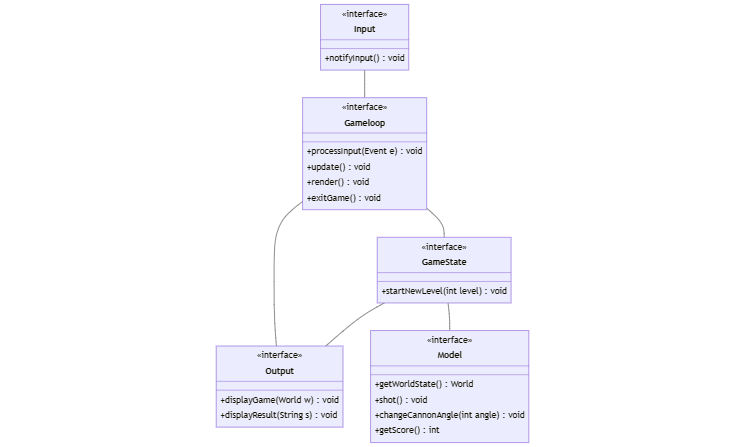
\includegraphics[width=\textwidth]{img/Diagramma_UML_Architettura}
\caption{Schema UML architetturale di Puzzle Bobble. Le interfacce \texttt{Gameloop e GameState} sono il controller del sistema, mentre \texttt{Input} ed \texttt{Output} sono le interfacce che mappano la view. \texttt{Model} è autoesplicativa.}
\label{img:Diagramma_UML_Architettura}
\end{figure}

In \Cref{img:Diagramma_UML_Architettura} è esemplificato il diagramma UML architetturale.

\newpage
\section{Design dettagliato}

In questa sezione si possono approfondire alcuni elementi del design con maggior dettaglio.
%
Mentre ci attendiamo principalmente (o solo) interfacce negli schemi UML delle sezioni precedenti,
in questa sezione è necessario scendere in maggior dettaglio presentando la struttura di alcune sottoparti rilevanti dell'applicazione.
%
È molto importante che, descrivendo la soluzione ad un problema, quando possibile si mostri che non si è re-inventata la ruota ma si è applicato un design pattern noto.
%
Che si sia utilizzato (o riconosciuto) o meno un pattern noto, è comunque bene definire qual è il problema che si è affrontato, qual è la soluzione messa in campo, e quali motivazioni l'hanno spinta.
%
È assolutamente inutile, ed è anzi controproducente, descrivere classe-per-classe (o peggio ancora metodo-per-metodo) com'è fatto il vostro software: è un livello di dettaglio proprio della documentazione dell'API (deducibile dalla Javadoc).

\textbf{È necessario che ciascun membro del gruppo abbia una propria sezione di design dettagliato,
di cui sarà il solo responsabile}.
%
Ciascun autore dovrà spiegare in modo corretto e giustamente approfondito (non troppo in dettaglio, non superficialmente) il proprio contributo.
%
È importante focalizzarsi sulle scelte che hanno un impatto positivo sul riuso, sull'estensibilità, e sulla chiarezza dell'applicazione.
%
Esattamente come nessun ingegnere meccanico presenta un solo foglio con l'intero progetto di una vettura di Formula 1, ma molteplici fogli di progetto che mostrano a livelli di dettaglio differenti le varie parti della vettura e le modalità di connessione fra le parti, così ci aspettiamo che voi, futuri ingegneri informatici, ci presentiate prima una visione globale del progetto, e via via siate in grado di dettagliare le singole parti, scartando i componenti che non interessano quella in esame.
%
Per continuare il parallelo con la vettura di Formula 1, se nei fogli di progetto che mostrano il
design delle sospensioni anteriori appaiono pezzi che appartengono al volante o al turbo, c'è una
chiara indicazione di qualche problema di design.

Si divida la sezione in sottosezioni, e per ogni aspetto di design che si vuole approfondire, si presenti:
\begin{enumerate}
    \item: una breve descrizione in linguaggio naturale del problema che si vuole risolvere, se necessario ci si può aiutare con schemi o immagini;
    \item: una descrizione della soluzione proposta, analizzando eventuali alternative che sono state prese in considerazione, e che descriva pro e contro della scelta fatta;
    \item: uno schema UML che aiuti a comprendere la soluzione sopra descritta;
    \item: se la soluzione è stata realizzata utilizzando uno o più pattern noti, si spieghi come questi sono reificati nel progetto
    (ad esempio: nel caso di Template Method, qual è il metodo template;
    nel caso di Strategy, quale interfaccia del progetto rappresenta la strategia, e quali sono le sue implementazioni;
    nel caso di Decorator, qual è la classe astratta che fa da Decorator e quali sono le sue implementazioni concrete; eccetera);
\end{enumerate}
%
La presenza di pattern di progettazione \emph{correttamente utilizzati} è valutata molto positivamente.
%
L'uso inappropriato è invece valutato negativamente: a tal proposito, si raccomanda di porre particolare attenzione all'abuso di Singleton, che, se usato in modo inappropriato, è di fatto un anti-pattern.

\subsection*{Elementi positivi}

\begin{itemize}
	\item Ogni membro del gruppo discute le proprie decisioni di progettazione, ed in particolare le azioni volte ad anticipare possibili cambiamenti futuri (ad esempio l'aggiunta di una nuova funzionalità, o il miglioramento di una esistente).
	\item Si mostrano le principali interazioni fra le varie componenti che collaborano alla soluzione di un determinato problema.
	\item Si identificano, utilizzano \textit{appropriatamente}, e descrivono diversi design pattern.
	\item Ogni membro del gruppo identifica i pattern utilizzati nella sua sottoparte.
	\item Si mostrano gli aspetti di design più rilevanti dell'applicazione, mettendo in luce la maniera in cui si è costruita la soluzione ai problemi descritti nell'analisi.
	\item Si tralasciano aspetti strettamente implementativi e quelli non rilevanti, non mostrandoli negli schemi UML (ad esempio, campi privati) e non descrivendoli.
	\item Ciascun elemento di design identificato presenta una piccola descrizione del problema calato
nell'applicazione, uno schema UML che ne mostra la concretizzazione nelle classi del progetto, ed
una breve descrizione della motivazione per cui tale soluzione è stata scelta, specialmente se è stato utilizzato un pattern noto. Ad esempio, se si
dichiara di aver usato Observer, è necessario specificare chi sia l'observable e chi l'observer; se
si usa Template Method, è necessario indicare quale sia il metodo template; se si usa Strategy, è
necessario identificare l'interfaccia che rappresenta la strategia; e via dicendo.
\end{itemize}

\subsection*{Elementi negativi}
\begin{itemize}
	\item Il design del modello risulta scorrelato dal problema descritto in analisi.
	\item Si tratta in modo prolisso, classe per classe, il software realizzato, o comunque si riduce la sezione ad un mero elenco di quanto fatto.
	\item Non si presentano schemi UML esemplificativi.
	\item Non si individuano design pattern, o si individuano in modo errato (si spaccia per design pattern qualcosa che non lo è).
	\item Si utilizzano design pattern in modo inopportuno. Un esempio classico è l'abuso di
Singleton per entità che possono essere univoche ma non devono necessariamente esserlo. Si rammenta
che Singleton ha senso nel secondo caso (ad esempio \texttt{System} e \texttt{Runtime} sono
singleton), mentre rischia di essere un problema nel secondo. Ad esempio, se si rendesse singleton
il motore di un videogioco, sarebbe impossibile riusarlo per costruire un server per partite online
(dove, presumibilmente, si gestiscono parallelamente più partite).
	\item Si producono schemi UML caotici e difficili da leggere, che comprendono inutili elementi di dettaglio.
	\item Si presentano schemi UML con classi (nel senso UML del termine) che ``galleggiano'' nello schema, non connesse, ossia senza relazioni con il resto degli elementi inseriti.
	\item Si tratta in modo inutilmente prolisso la divisione in package, elencando ad esempio le classi una per una.
\end{itemize}

\subsection*{Esempio minimale (e quindi parziale) di sezione di progetto con UML ben realizzati}

\subsubsection{Personalità intercambiabili}

\begin{figure}[H]
\centering{}
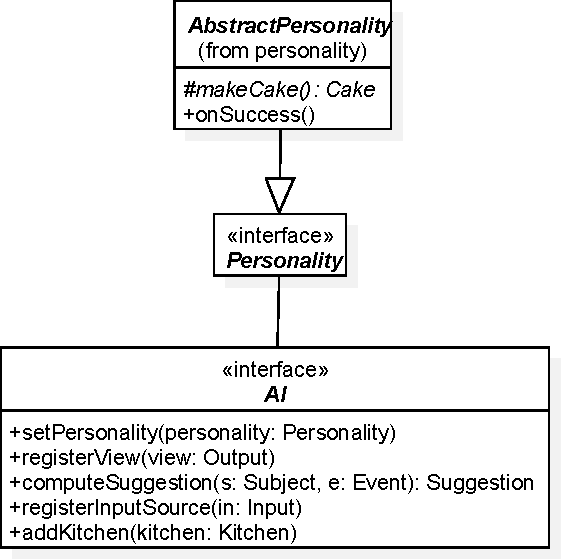
\includegraphics[width=\textwidth]{img/strategy}
\caption{Rappresentazione UML del pattern Strategy per la personalità di GLaDOS}
\label{img:strategy}
\end{figure}

\paragraph{Problema} GLaDOS ha più personalità intercambiabili, la cui presenza deve essere trasparente al client.

\paragraph{Soluzione} Il sistema per la gestione della personalità utilizza il \textit{pattern Strategy}, come da
\Cref{img:strategy}: le implementazioni di \texttt{Personality} possono essere modificate, e la
modifica impatta direttamente sul comportamento di GLaDOS.

\subsubsection{Riuso del codice delle personalità}

\begin{figure}[H]
\centering{}
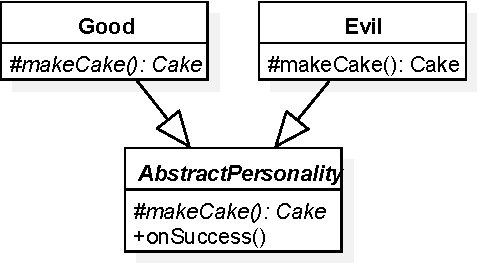
\includegraphics[width=\textwidth]{img/template}
\caption{Rappresentazione UML dell'applicazione del pattern Template Method alla gerarchia delle Personalità}
\label{img:template}
\end{figure}

\paragraph{Problema} In fase di sviluppo, sono state sviluppate due personalità, una buona ed una cattiva.
Quella buona restituisce sempre una torta vera, mentre quella cattiva restituisce sempre la
promessa di una torta che verrà in realtà disattesa.
Ci si è accorti che diverse personalità condividevano molto del comportamento,
portando a classi molto simili e a duplicazione.

\paragraph{Soluzione} Dato che le due personalità differiscono solo per il comportamento da effettuarsi in caso di percorso completato con successo,
è stato utilizzato il \textit{pattern template method} per massimizzare il riuso, come da \Cref{img:template}.
Il metodo template è \texttt{onSuccess()}, che chiama un metodo astratto e protetto
\texttt{makeCake()}.

\subsubsection{Gestione di output multipli}

\begin{figure}[H]
\centering{}
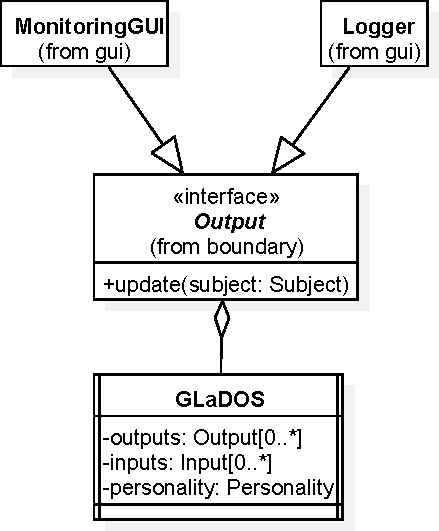
\includegraphics[width=.7\textwidth]{img/observer}
\caption{Il pattern Observer è usato per consentire a GLaDOS di informare tutti i sistemi di output in ascolto}
\label{img:observer}
\end{figure}

\paragraph{Problema} Il sistema deve supportare output multipli. In particolare, si richiede che vi sia un logger che stampa a terminale o su file,
e un'interfaccia grafica che mostri una rappresentazione grafica del sistema.

\paragraph{Soluzione} Dato che i due sistemi di reporting utilizzano le medesime informazioni, si è deciso di raggrupparli dietro l'interfaccia \texttt{Output}.
A questo punto, le due possibilità erano quelle di far sì che \texttt{GLaDOS} potesse pilotarle entrambe.
Invece di fare un sistema in cui questi output sono obbligatori e connessi, si è deciso di usare maggior flessibilità (anche in vista di future estensioni)
e di adottare una comunicazione uno-a-molti fra \texttt{GLaDOS} ed i sistemi di output.
La scelta è quindi ricaduta sul \textit{pattern Observer}: \texttt{GLaDOS} è observable, e le istanze di \texttt{Output} sono observer.
%
Il suo utilizzo è esemplificato in \Cref{img:observer}


\subsection*{Contro-esempio: pessimo diagramma UML}

In \Cref{img:badarch} è mostrato il modo \textbf{sbagliato} di fare le cose.
%
Questo schema è fatto male perché:
\begin{itemize}
	\item È caotico.
	\item È difficile da leggere e capire.
	\item Vi sono troppe classi, e non si capisce bene quali siano i rapporti che intercorrono fra loro.
	\item Si mostrano elementi implementativi irrilevanti, come i campi e i metodi privati nella classe \texttt{AbstractEnvironment}.
	\item Se l'intenzione era quella di costruire un diagramma architetturale, allora lo schema è ancora più sbagliato, perché mostra pezzi di implementazione.
	\item Una delle classi, in alto al centro, galleggia nello schema, non connessa a nessuna altra classe, e di fatto costituisce da sola un secondo schema UML scorrelato al resto
	\item Le interfacce presentano tutti i metodi e non una selezione che aiuti il lettore a capire quale parte del sistema si vuol mostrare.
\end{itemize}


\begin{figure}[h]
\centering{}
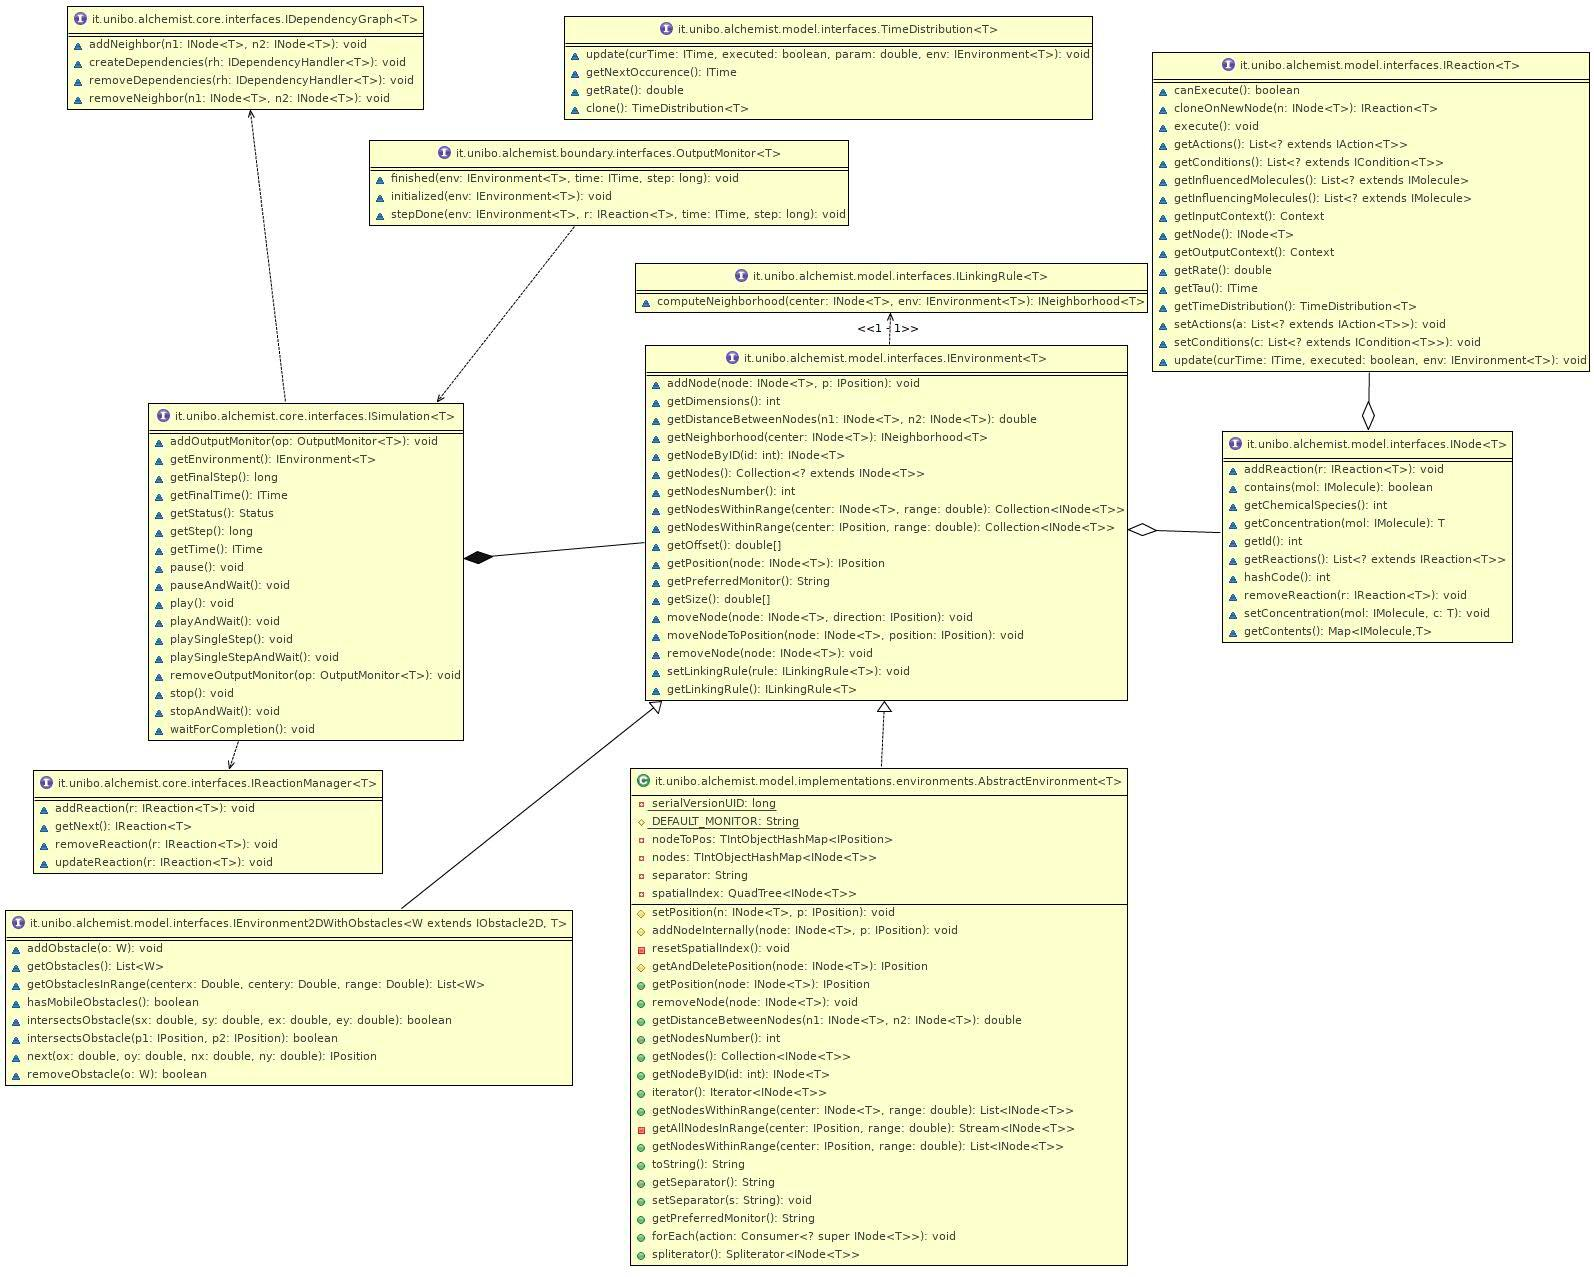
\includegraphics[width=\textwidth]{img/badarch}
\caption{Schema UML mal fatto e con una pessima descrizione, che non aiuta a capire. Don't try this at home.}
\label{img:badarch}
\end{figure}


\chapter{Sviluppo}
\section{Testing automatizzato}

Il testing automatizzato è un requisito di qualunque progetto software che si rispetti, e consente di verificare che non vi siano regressioni nelle funzionalità a fronte di aggiornamenti.
%
Per quanto riguarda questo progetto è considerato sufficiente un test minimale, a patto che sia completamente automatico.
%
Test che richiedono l'intervento da parte dell'utente sono considerati \textit{negativamente} nel computo del punteggio finale.

\subsection*{Elementi positivi}

\begin{itemize}
 \item Si descrivono molto brevemente i componenti che si è deciso di sottoporre a test automatizzato.
 \item Si utilizzano suite specifiche (e.g. JUnit) per il testing automatico.
\end{itemize}

\subsection*{Elementi negativi}
\begin{itemize}
 \item Non si realizza alcun test automatico.
 \item La non presenza di testing viene aggravata dall'adduzione di motivazioni non valide. Ad esempio, si scrive che l'interfaccia grafica non è testata automaticamente perché è \emph{impossibile} farlo\footnote{Testare in modo automatico le interfacce grafiche è possibile (si veda, come esempio, \url{https://github.com/TestFX/TestFX}), semplicemente nel corso non c'è modo e tempo di introdurvi questo livello di complessità. Il fatto che non vi sia stato insegnato come farlo non implica che sia impossibile!}.
 \item Si descrive un testing di tipo manuale in maniera prolissa.
 \item Si descrivono test effettuati manualmente che sarebbero potuti essere automatizzati, ad esempio scrivendo che si è usata l'applicazione manualmente.
 \item Si descrivono test non presenti nei sorgenti del progetto.
 \item I test, quando eseguiti, falliscono.
\end{itemize}

\section{Metodologia di lavoro}

Ci aspettiamo, leggendo questa sezione, di trovare conferma alla divisione operata nella sezione del design di dettaglio, e di capire come è stato svolto il lavoro di integrazione.
%
\textbf{Andrà realizzata una sotto-sezione separata per ciascuno studente} che identifichi le porzioni di progetto sviluppate, separando quelle svolte in autonomia da quelle sviluppate in collaborazione.
%
Diversamente dalla sezione di design, in questa è consentito elencare package/classi, se lo studente ritiene sia il modo più efficace di convogliare l'informazione.
%
Si ricorda che l'impegno deve giustificare circa 40-50 ore di sviluppo (è normale e fisiologico che approssimativamente la metà del tempo sia impiegata in analisi e progettazione).

\subsection*{Elementi positivi}

\begin{itemize}
	\item Si identifica con precisione il ruolo di ciascuno all'interno del gruppo, ossia su quale parte del progetto ciascuno dei componenti si è concentrato maggiormente.
	\item La divisione dei compiti è equa, ossia non vi sono membri del gruppo che hanno svolto molto più lavoro di altri.
	\item La divisione dei compiti è coerente con quanto descritto nelle parti precedenti della relazione.
	\item La divisione dei compiti è realistica, ossia le dipendenze fra le parti sviluppate sono minime.
	\item Si identifica quale parte del software è stato sviluppato da tutti i componenti insieme.
	\item Si spiega in che modo si sono integrate le parti di codice sviluppate separatamente, evidenziando eventuali problemi. Ad esempio, una strategia è convenire sulle interfacce da usare (ossia, occuparsi insieme di stabilire l'architettura) e quindi procedere indipendentemente allo sviluppo di parti differenti. Una possibile problematica potrebbe essere una dimenticanza in fase di design architetturale che ha costretto ad un cambio e a modifiche in fase di integrazione. Una situazione simile è la norma nell'ingegneria di un sistema software non banale, ed il processo di progettazione top-down con raffinamento successivo è il così detto processo ``a spirale''.
	\item Si descrive in che modo è stato impiegato il DVCS.
\end{itemize}

\subsection*{Elementi negativi}
\begin{itemize}
	\item Non si chiarisce chi ha fatto cosa.
	\item C'è discrepanza fra questa sezione e le sezioni che descrivono il design dettagliato.
	\item Tutto il progetto è stato svolto lavorando insieme invece che assegnando una parte a ciascuno.
	\item Non viene descritta la metodologia di integrazione delle parti sviluppate indipendentemente.
	\item Uso superficiale del DVCS.
\end{itemize}

\section{Note di sviluppo}

Questa sezione, come quella riguardante il design dettagliato va svolta \textbf{singolarmente da ogni membro del gruppo}.
%
Nella prima parte, ciascuno dovrà mostrare degli esempi di codice particolarmente ben realizzati,
che dimostrino proefficienza con funzionalità avanzate del linguaggio e capacità di spingersi oltre le librerie mostrate a lezione.

\begin{itemize}
	\item \textbf{Elencare} (fare un semplice elenco per punti, non un testo!) le feature \textit{avanzate} del linguaggio e dell'ecosistema Java che sono state
utilizzate. Le feature di interesse sono:
	\begin{itemize}
		\item Progettazione con generici, ad esempio costruzione di nuovi tipi generici, e uso di generici bounded.
		L'uso di classi generiche di libreria non è considerato avanzato.
		\item Uso di lambda expressions
		\item Uso di \texttt{Stream}, di \texttt{Optional} o di altri costrutti funzionali
		\item Uso di reflection
		\item Definizione ed uso di nuove annotazioni
		\item Uso del Java Platform Module System
		\item Uso di parti della libreria JDK non spiegate a lezione (networking, compressione, parsing XML, eccetera...)
		\item Uso di librerie di terze parti (incluso JavaFX): Google Guava, Apache Commons...
	\end{itemize}
	\item Si faccia molta attenzione a non scrivere banalità, elencando qui features di tipo ``core'', come le eccezioni, le enumerazioni, o le inner class: nessuna di queste è considerata avanzata.
	\item Per ogni feature avanzata, mostrata, includere:
	\begin{itemize}
		\item Nome della feature
		\item Permalink GitHub al punto nel codice in cui è stata utilizzata
	\end{itemize}
\end{itemize}

In questa sezione, \textit{dopo l'elenco},
vanno menzionati ed attributi con precisione eventuali pezzi di codice ``riadattati'' (o scopiazzati...) da Internet o da altri progetti,
pratica che tolleriamo ma che non raccomandiamo.
%
Si rammenta agli studenti che non è consentito partire da progetti esistenti e procedere per modifiche successive.
%
Si ricorda anche che i docenti hanno in mano strumenti antiplagio piuttosto raffinati e che ``capiscono'' il codice e la storia delle modifiche del progetto,
per cui tecniche banali come cambiare nomi (di classi, metodi, campi, parametri, o variabili locali),
aggiungere o togliere commenti,
oppure riordinare i membri di una classe vengono individuate senza problemi.
%
Le regole del progetto spiegano in dettaglio l'approccio dei docenti verso atti gravi come il plagiarismo.

I pattern di design \textbf{non} vanno messi qui.
%
L'uso di pattern di design (come suggerisce il nome) è un aspetto avanzato di design, non di implementazione,
e non va in questa sezione.

\subsection*{Elementi positivi}

\begin{itemize}
	\item Si elencano gli aspetti avanzati di linguaggio che sono stati impiegati
	\item Si elencano le librerie che sono state utilizzate
	\item Per ciascun elemento, si fornisce un permalink
	\item Ogni permalink fa riferimento ad uno snippet di codice scritto dall'autore della sezione (i docenti verificheranno usando \texttt{git blame})
	\item Se si è utilizzato un particolare algoritmo, se ne cita la fonte originale.
	Ad esempio, se si è usato Mersenne Twister per la generazione di numeri pseudo-random, si cita \cite{mersenne}.
	\item Si identificano parti di codice prese da altri progetti, dal web, o comunque scritte in forma originale da altre persone.
	In tal senso, si ricorda che agli ingegneri non è richiesto di re-inventare la ruota continuamente:
	se si cita debitamente la sorgente è tollerato fare uso di di snippet di codice open source per risolvere velocemente problemi non banali.
	Nel caso in cui si usino snippet di codice di qualità discutibile,
	oltre a menzionarne l'autore originale si invitano gli studenti ad adeguare tali parti di codice agli standard e allo stile del progetto.
	Contestualmente, si fa presente che è largamente meglio fare uso di una libreria che copiarsi pezzi di codice:
	qualora vi sia scelta (e tipicamente c'è), si preferisca la prima via.
\end{itemize}

\subsection*{Elementi negativi}
\begin{itemize}
	\item Si elencano feature core del linguaggio invece di quelle segnalate. Esempi di feature core da non menzionare sono:
    \begin{itemize}
        \item eccezioni;
        \item classi innestate;
        \item enumerazioni;
        \item interfacce.
    \end{itemize}
	\item Si elencano applicazioni di terze parti (peggio se per usarle occorre licenza, e lo studente ne è sprovvisto) che non c'entrano nulla con lo sviluppo, ad esempio:
    \begin{itemize}
        \item Editor di grafica vettoriale come Inkscape o Adobe Illustrator;
        \item Editor di grafica scalare come GIMP o Adobe Photoshop;
        \item Editor di audio come Audacity;
        \item Strumenti di design dell'interfaccia grafica come SceneBuilder: il codice è in ogni caso inteso come sviluppato da voi.
    \end{itemize}
	\item Si descrivono aspetti di scarsa rilevanza, o si scende in dettagli inutili.
	\item Sono presenti parti di codice sviluppate originalmente da altri che non vengono debitamente segnalate.
	In tal senso, si ricorda agli studenti che i docenti hanno accesso a tutti i progetti degli anni passati,
	a Stack Overflow,
	ai principali blog di sviluppatori ed esperti Java,
	ai blog dedicati allo sviluppo di soluzioni e applicazioni
	(inclusi blog dedicati ad Android e allo sviluppo di videogame),
	nonché ai vari GitHub, GitLab, e Bitbucket.
	Conseguentemente, è \emph{molto} conveniente \emph{citare} una fonte ed usarla invece di tentare di spacciare per proprio il lavoro di altri.
	\item Si elencano design pattern
\end{itemize}

\subsection{Esempio}

\subsubsection{Utilizzo della libreria SLF4J}

Utilizzata in vari punti.
Un esempio è \url{https://github.com/AlchemistSimulator/Alchemist/blob/5c17f8b76920c78d955d478864ac1f11508ed9ad/alchemist-swingui/src/main/java/it/unibo/alchemist/boundary/swingui/effect/impl/EffectBuilder.java#L49}

\subsubsection{Utilizzo di \texttt{LoadingCache} dalla libreria Google Guava}

Permalink: \url{https://github.com/AlchemistSimulator/Alchemist/blob/d8a1799027d7d685569e15316a32e6394632ce71/alchemist-incarnation-protelis/src/main/java/it/unibo/alchemist/protelis/AlchemistExecutionContext.java#L141-L143}

\subsubsection{Utilizzo di \texttt{Stream} e lambda expressions}

Usate pervasivamente. Il seguente è un singolo esempio.
Permalink: \url{https://github.com/AlchemistSimulator/Alchemist/blob/d8a1799027d7d685569e15316a32e6394632ce71/alchemist-incarnation-protelis/src/main/java/it/unibo/alchemist/model/ProtelisIncarnation.java#L98-L120}

\subsubsection{Scrittura di metodo generico con parametri contravarianti}

Permalink: \url{https://github.com/AlchemistSimulator/Alchemist/blob/d8a1799027d7d685569e15316a32e6394632ce71/alchemist-incarnation-protelis/src/main/java/it/unibo/alchemist/protelis/AlchemistExecutionContext.java#L141-L143}

\subsubsection{Protezione da corse critiche usando \texttt{Semaphore}}

Permalink: \url{https://github.com/AlchemistSimulator/Alchemist/blob/d8a1799027d7d685569e15316a32e6394632ce71/alchemist-incarnation-protelis/src/main/java/it/unibo/alchemist/model/ProtelisIncarnation.java#L388-L440}


\chapter{Commenti finali}

In quest'ultimo capitolo si tirano le somme del lavoro svolto e si delineano eventuali sviluppi
futuri.

\textit{Nessuna delle informazioni incluse in questo capitolo verrà utilizzata per formulare la valutazione finale}, a meno che non sia assente o manchino delle sezioni obbligatorie.
%
Al fine di evitare pregiudizi involontari, l'intero capitolo verrà letto dai docenti solo dopo aver formulato la valutazione.

\section{Autovalutazione e lavori futuri}

\textbf{È richiesta una sezione per ciascun membro del gruppo, obbligatoriamente}.
%
Ciascuno dovrà autovalutare il proprio lavoro, elencando i punti di forza e di debolezza in quanto prodotto.
Si dovrà anche cercare di descrivere \emph{in modo quanto più obiettivo possibile} il proprio ruolo all'interno del gruppo.
Si ricorda, a tal proposito, che ciascuno studente è responsabile solo della propria sezione: non è un problema se ci sono opinioni contrastanti, a patto che rispecchino effettivamente l'opinione di chi le scrive.
Nel caso in cui si pensasse di portare avanti il progetto, ad esempio perché effettivamente impiegato, o perché sufficientemente ben riuscito da poter esser usato come dimostrazione di esser capaci progettisti, si descriva brevemente verso che direzione portarlo.

\section{Difficoltà incontrate e commenti per i docenti}

Questa sezione, \textbf{opzionale}, può essere utilizzata per segnalare ai docenti eventuali problemi o difficoltà incontrate nel corso o nello svolgimento del progetto, può essere vista come una seconda possibilità di valutare il corso (dopo quella offerta dalle rilevazioni della didattica) avendo anche conoscenza delle modalità e delle difficoltà collegate all'esame, cosa impossibile da fare usando le valutazioni in aula per ovvie ragioni.
%
È possibile che alcuni dei commenti forniti vengano utilizzati per migliorare il corso in futuro: sebbene non andrà a vostro beneficio, potreste fare un favore ai vostri futuri colleghi.
%
Ovviamente \textit{il contenuto della sezione non impatterà il voto finale}.

\appendix
\chapter{Guida utente}

Capitolo in cui si spiega come utilizzare il software. Nel caso in cui il suo uso sia del tutto
banale, tale capitolo può essere omesso.
%
A tal riguardo, si fa presente agli studenti che i docenti non hanno mai utilizzato il software
prima, per cui aspetti che sembrano del tutto banali a chi ha sviluppato l'applicazione possono non
esserlo per chi la usa per la prima volta.
%
Se, ad esempio, per cominciare una partita con un videogioco è necessario premere la barra
spaziatrice, o il tasto ``P'', è necessario che gli studenti lo segnalino.

\subsection*{Elementi positivi}

\begin{itemize}
 \item Si istruisce in modo semplice l'utente sull'uso dell'applicazione, eventualmente facendo uso di schermate e descrizioni.
\end{itemize}

\subsection*{Elementi negativi}
\begin{itemize}
 \item Si descrivono in modo eccessivamente minuzioso tutte le caratteristiche, anche minori, del software in oggetto.
 \item Manca una descrizione che consenta ad un utente qualunque di utilizzare almeno le funzionalità primarie dell'applicativo.
\end{itemize}

\chapter{Esercitazioni di laboratorio}

In questo capitolo ciascuno studente elenca gli esercizi di laboratorio che ha svolto
(se ne ha svolti),
elencando i permalink dei post sul forum dove è avvenuta la consegna.
%
Questa sezione potrebbe essere processata da strumenti automatici,
per cui link a oggetti diversi dal permalink della consegna,
errori nell'email o nel nome del laboratorio possono portare ad ignorare alcune consegne,
si raccomanda la massima precisione.

\section*{Esempio}

\subsection{paolino.paperino@studio.unibo.it}

\begin{itemize}
 \item Laboratorio 04: \url{https://virtuale.unibo.it/mod/forum/discuss.php?d=12345#p123456}
 \item Laboratorio 06: \url{https://virtuale.unibo.it/mod/forum/discuss.php?d=22222#p222222}
 \item Laboratorio 09: \url{https://virtuale.unibo.it/mod/forum/discuss.php?d=99999#p999999}
\end{itemize}

\subsection{paperon.depaperoni@studio.unibo.it}

\begin{itemize}
 \item Laboratorio 04: \url{https://virtuale.unibo.it/mod/forum/discuss.php?d=12345#p123456}
 \item Laboratorio 05: \url{https://virtuale.unibo.it/mod/forum/discuss.php?d=22222#p222222}
 \item Laboratorio 06: \url{https://virtuale.unibo.it/mod/forum/discuss.php?d=99999#p999999}
 \item Laboratorio 07: \url{https://virtuale.unibo.it/mod/forum/discuss.php?d=22222#p222222}
 \item Laboratorio 08: \url{https://virtuale.unibo.it/mod/forum/discuss.php?d=99999#p999999}
 \item Laboratorio 09: \url{https://virtuale.unibo.it/mod/forum/discuss.php?d=22222#p222222}
 \item Laboratorio 10: \url{https://virtuale.unibo.it/mod/forum/discuss.php?d=99999#p999999}
 \item Laboratorio 11: \url{https://virtuale.unibo.it/mod/forum/discuss.php?d=22222#p222222}
\end{itemize}


\bibliographystyle{alpha}
\bibliography{13-template}

\end{document}
